%%%%
% Преамбула: подключение необходимых пакетов
% Редактируйте осторожно!
%

\documentclass[hyperref={unicode}]{beamer}

\usepackage[utf8x]{inputenc}
\usepackage[english, russian]{babel}
\usepackage{color, colortbl}
\usepackage{rotating} 
\usepackage{graphicx}
\usepackage{algorithmic}
\usepackage[font=footnotesize,labelfont=bf]{caption}

\setbeamertemplate{caption}[numbered]
\usetheme[nosecheader]{PetrSU-CS}


%%%%
% Преамбула: основные параметры презентации
% Отредактируйте в соответствии с комментариями
%

\title[%
	% Краткое название работы не используется в этой презентации!
		Клиент веб-сервиса для коллективных переводов
]{%
		% Полное название работы отображается на титульной странице
		Разработка клиентской части веб-сервиса для коллективных переводов
}

% Подзаголовком опишите тип работы:
% - Курсовая работа
% - Выпускная квалификационная работа бакалавра
% - Дипломная работа
% - Магистерская диссертация
\subtitle{Отчет о научно-исследовательской работе}

\author[%
		% Имя и фамилия автора работы отображаются на каждом слайде в нижнем колонтитуле
		Зименкова Софья
]{%
		% Имя, отчество и фамилия автора работы отображаются на титульном слайде
		Зименкова Софья Эдуардовна
}

\date[%
		% Дата защиты
		10.04.2024
]{%
		% Руководитель
		Научный руководитель: Д. Б. Чистяков
}

\institute[%
		% Краткое название организации не используется в этой презентации
		ПетрГУ
]{%
		% Полное название организации и подразделения
		Петрозаводский государственный университет\\
		Кафедра Информатики и Математического Обеспечения
}


%%%%
%
% Начало содержимого слайдов
%


%\begin{center}
%	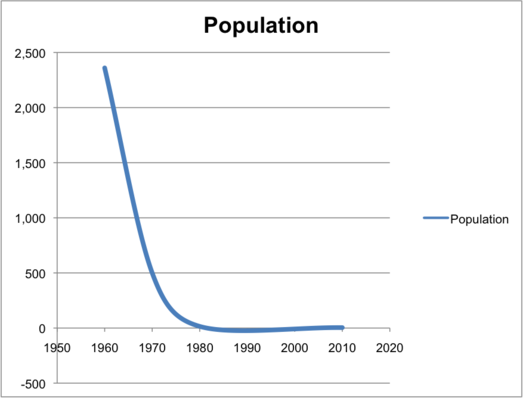
\includegraphics[width=0.4\textwidth]{images/pop.png}
%\end{center

\begin{document}

% Титульный слайд
\begin{frame}
\maketitle
\end{frame}


\begin{frame}
	\frametitle{Актуальность и требования к сервису}
	Для организации эффективной работы коллектива переводчиков инструмент должен иметь следующие фукнции:
 \begin{itemize}
		\item Загрузка текста и определение участников его перевода;
		\item Разбиение исходного текста на главы и фрагменты;
		\item Синхронизация материалов и прогресса между участниками перевода;
		\item Поиск существующих в системе переводов;
		\item Выбор и утверждение наилучшего варианта перевода;
		\item Выгрузка итогового текста.
	\end{itemize}
	Существующие сервисы, предоставляющие переводчикам эти и похожие функции, не подходят для работы команды волонтеров, поскольку являются коммерческими сервисами или сильно устарели и не поддерживаются.
\end{frame}


\begin{frame}
	\frametitle{Цель и задачи}
	\begin{block}{Цель работы}
		Разработать клиентскую часть веб-сервиса для коллективных переводов.
	\end{block}
	\begin{block}{Задачи}
	\begin{itemize}
		\item Сформулировать требования к клиентской части веб-сервиса;
		\item Разработать проект клиентской части веб-сервиса;
		\item Разработать макет пользовательского интерфейса;
		\item Разработать и интегрировать клиентскую часть веб-сервиса в информационную систему.
	\end{itemize}
	\end{block}
\end{frame}


\begin{frame}
	\frametitle{Проектирование веб-сервиса}
	\begin{figure}
	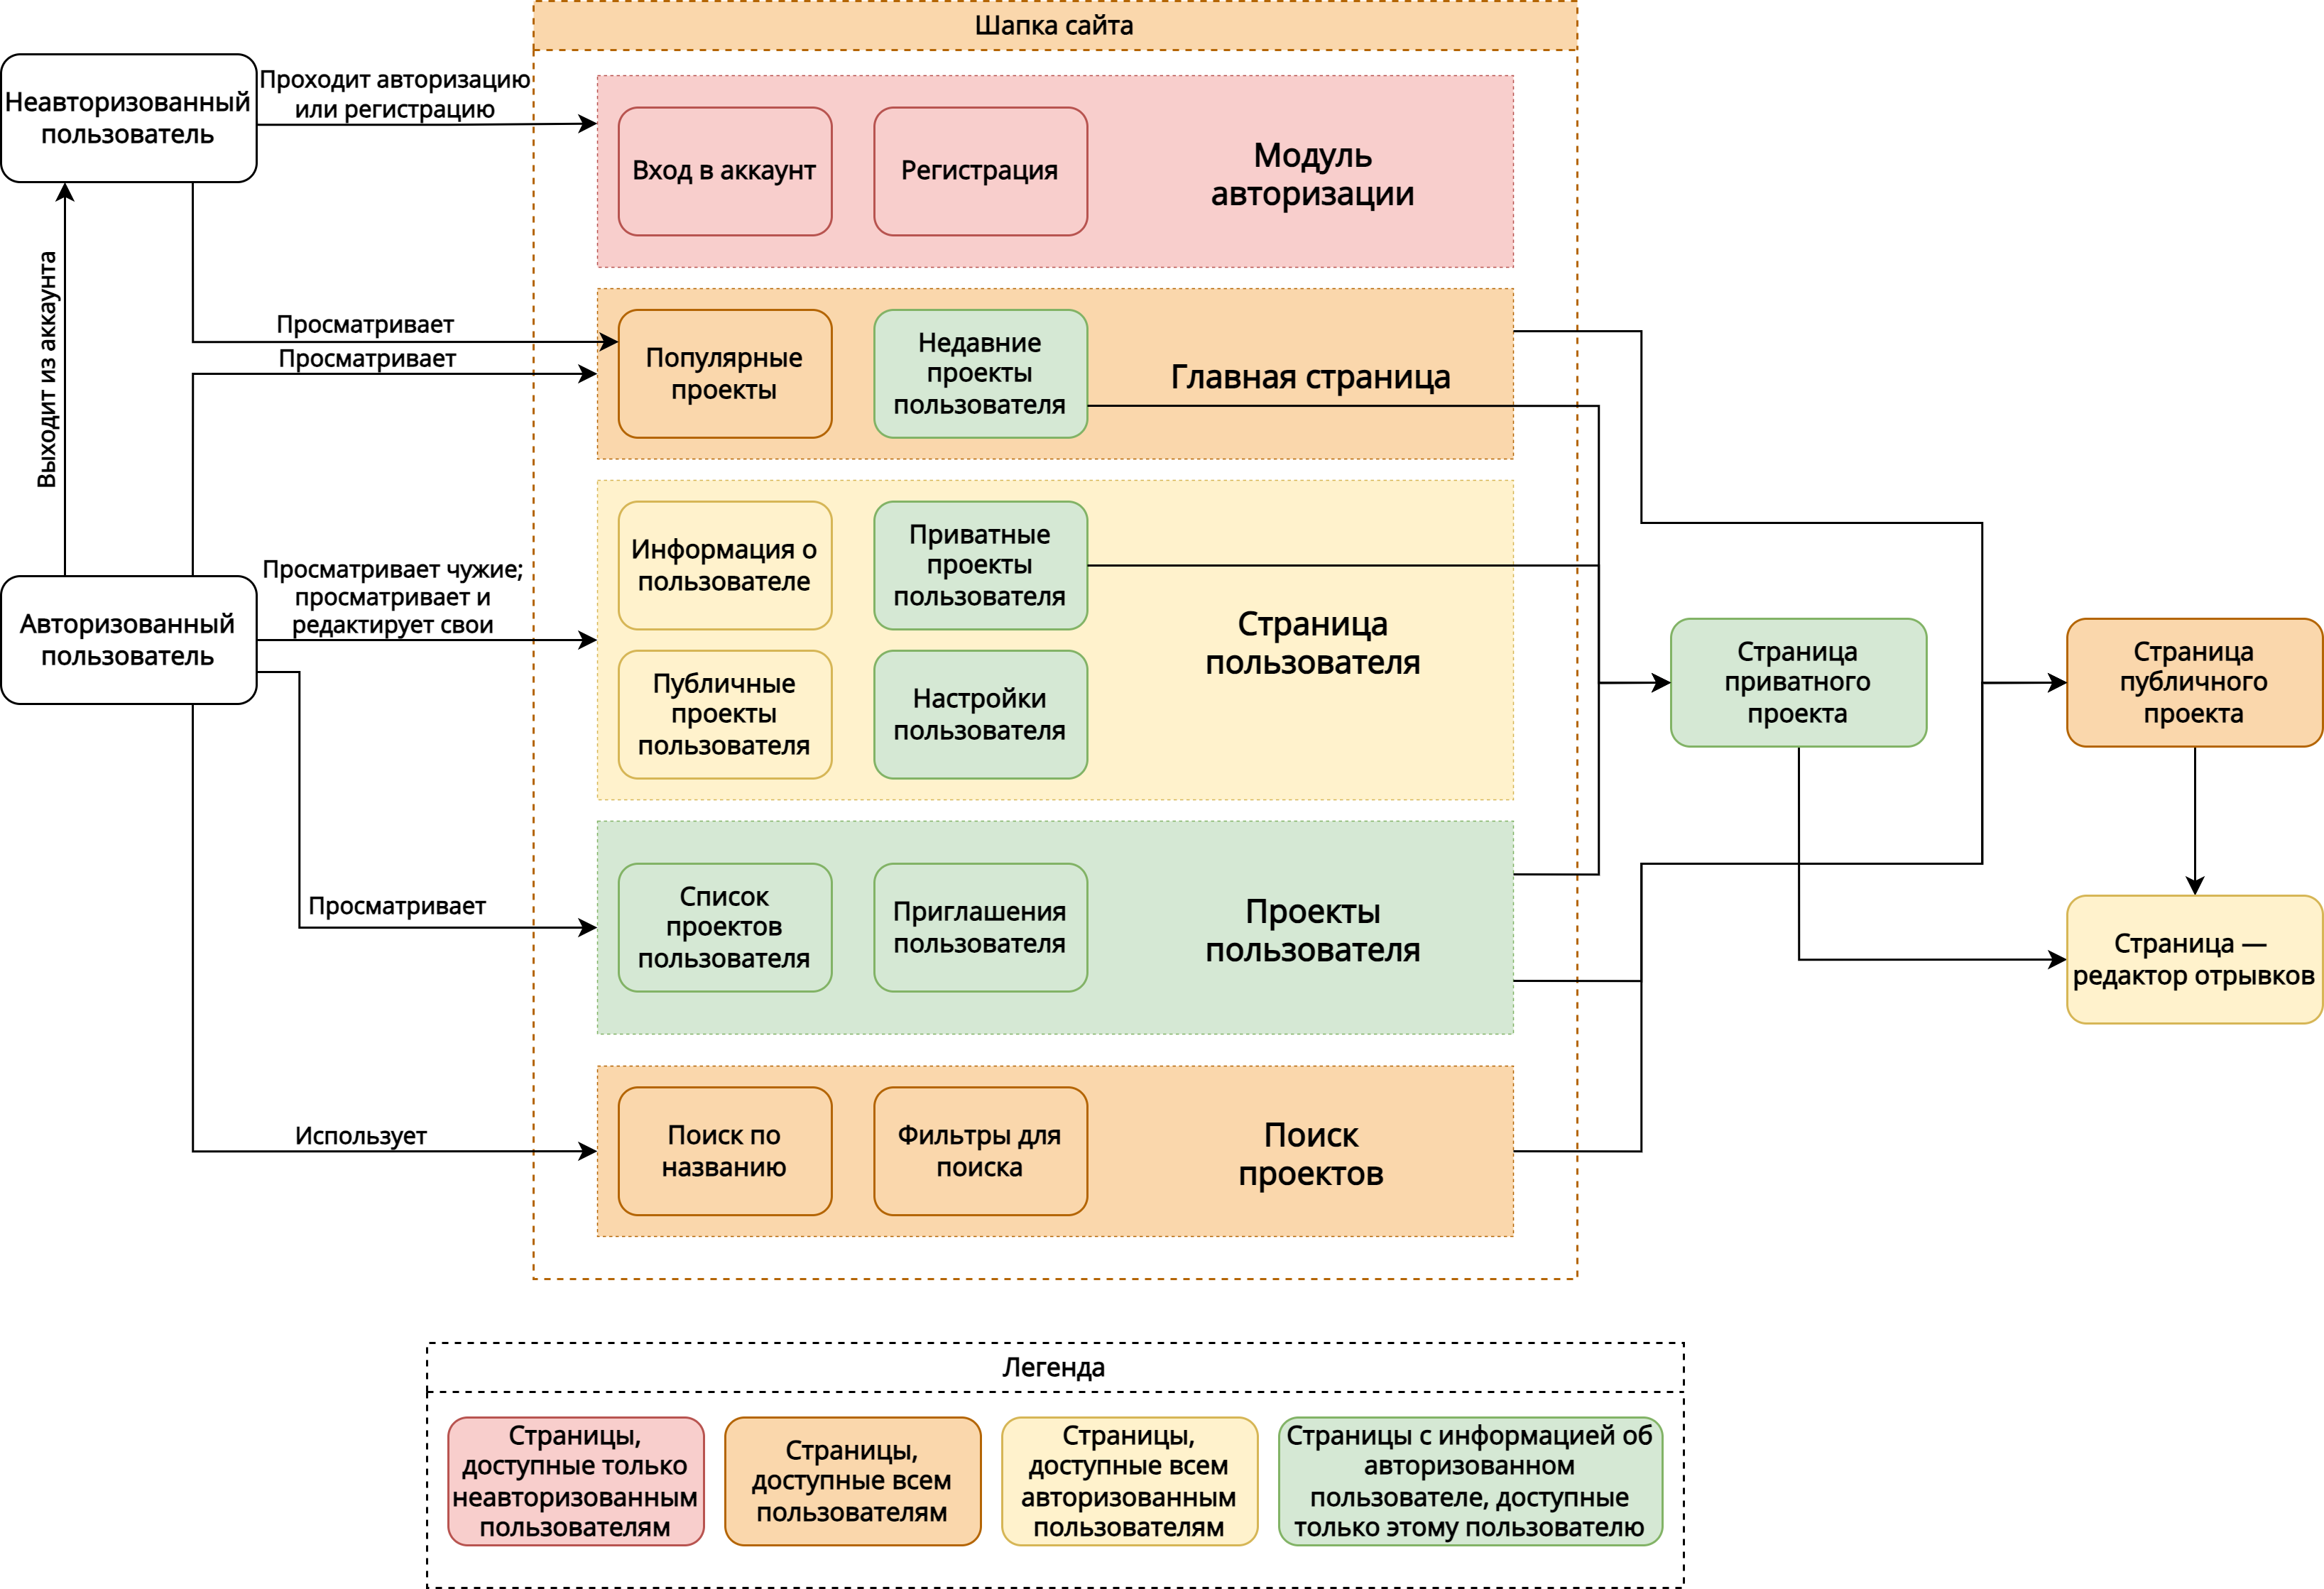
\includegraphics[width=300px]{images/pagesdiagram1.png}
	\caption{Диаграмма процессов предметной области: навигация по веб-сайту}
	\end{figure}
\end{frame}


\begin{frame}
	\frametitle{Проектирование веб-сервиса}
	\begin{figure}
	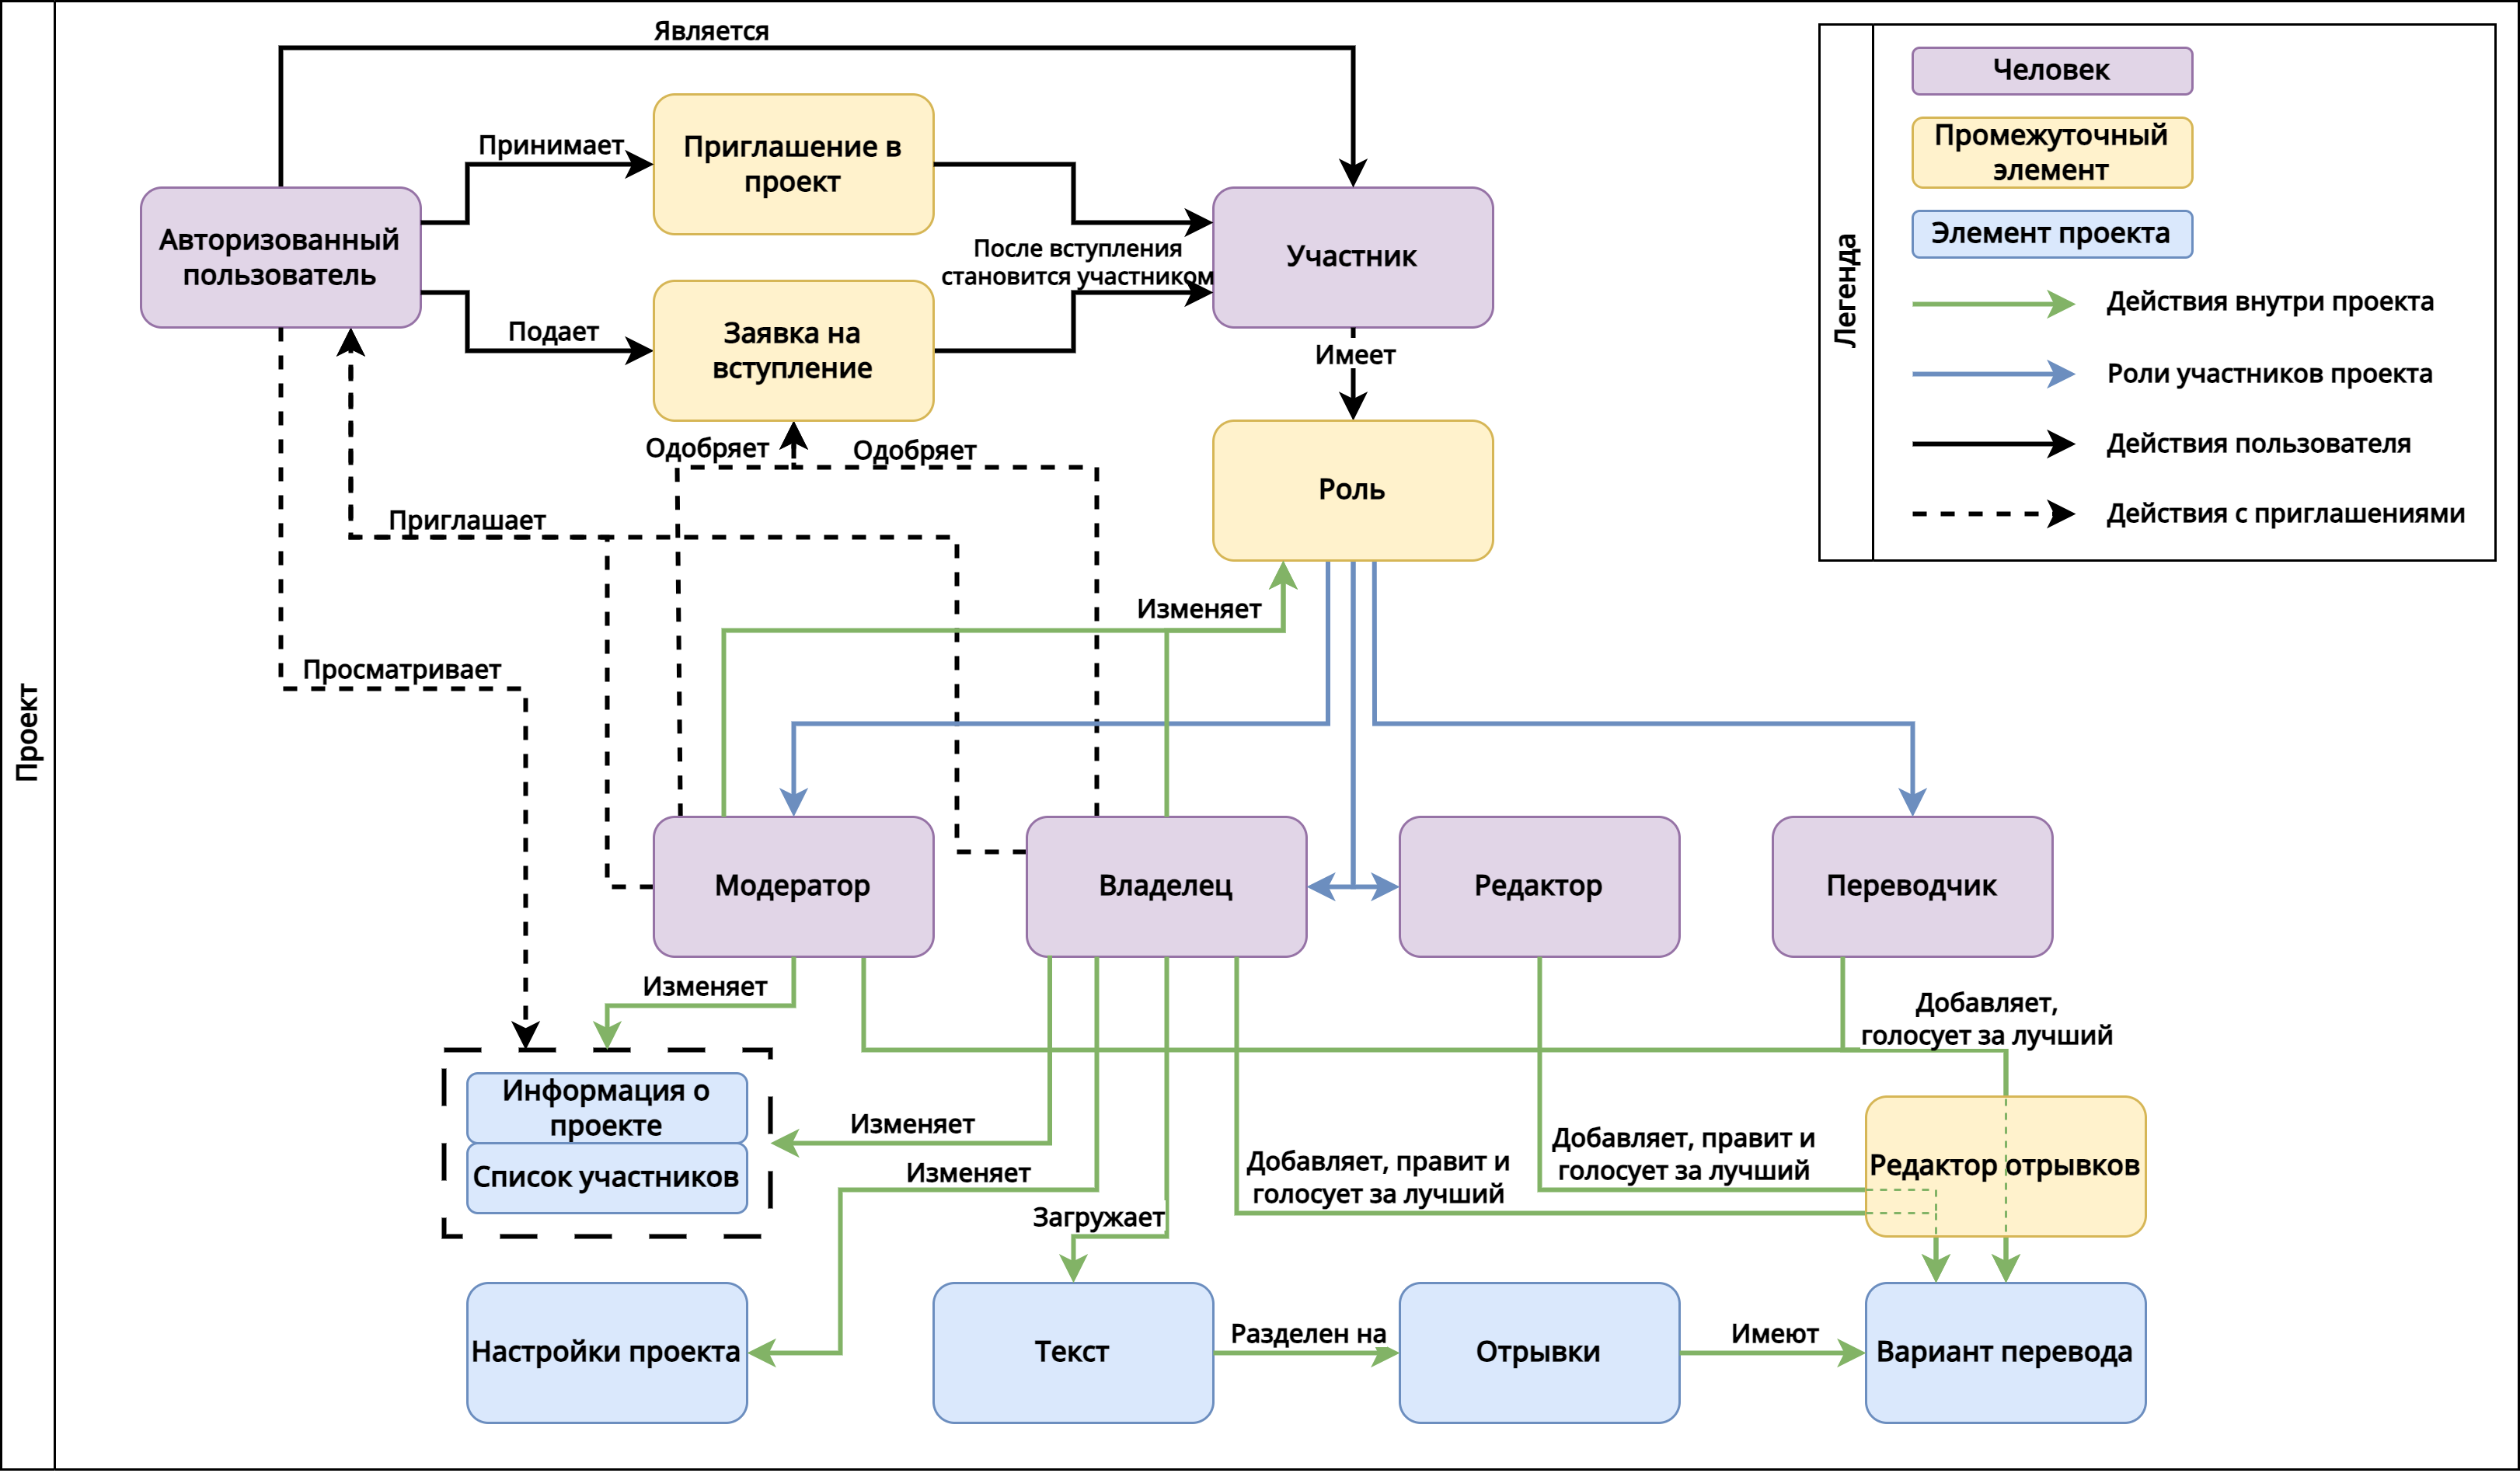
\includegraphics[width=\textwidth]{images/pagesdiagram2.png}
	\caption{Диаграмма процессов предметной области: структура проекта}
	\end{figure}
\end{frame}


\begin{frame}
	\frametitle{Проектирование веб-сервиса}
	\begin{figure}
	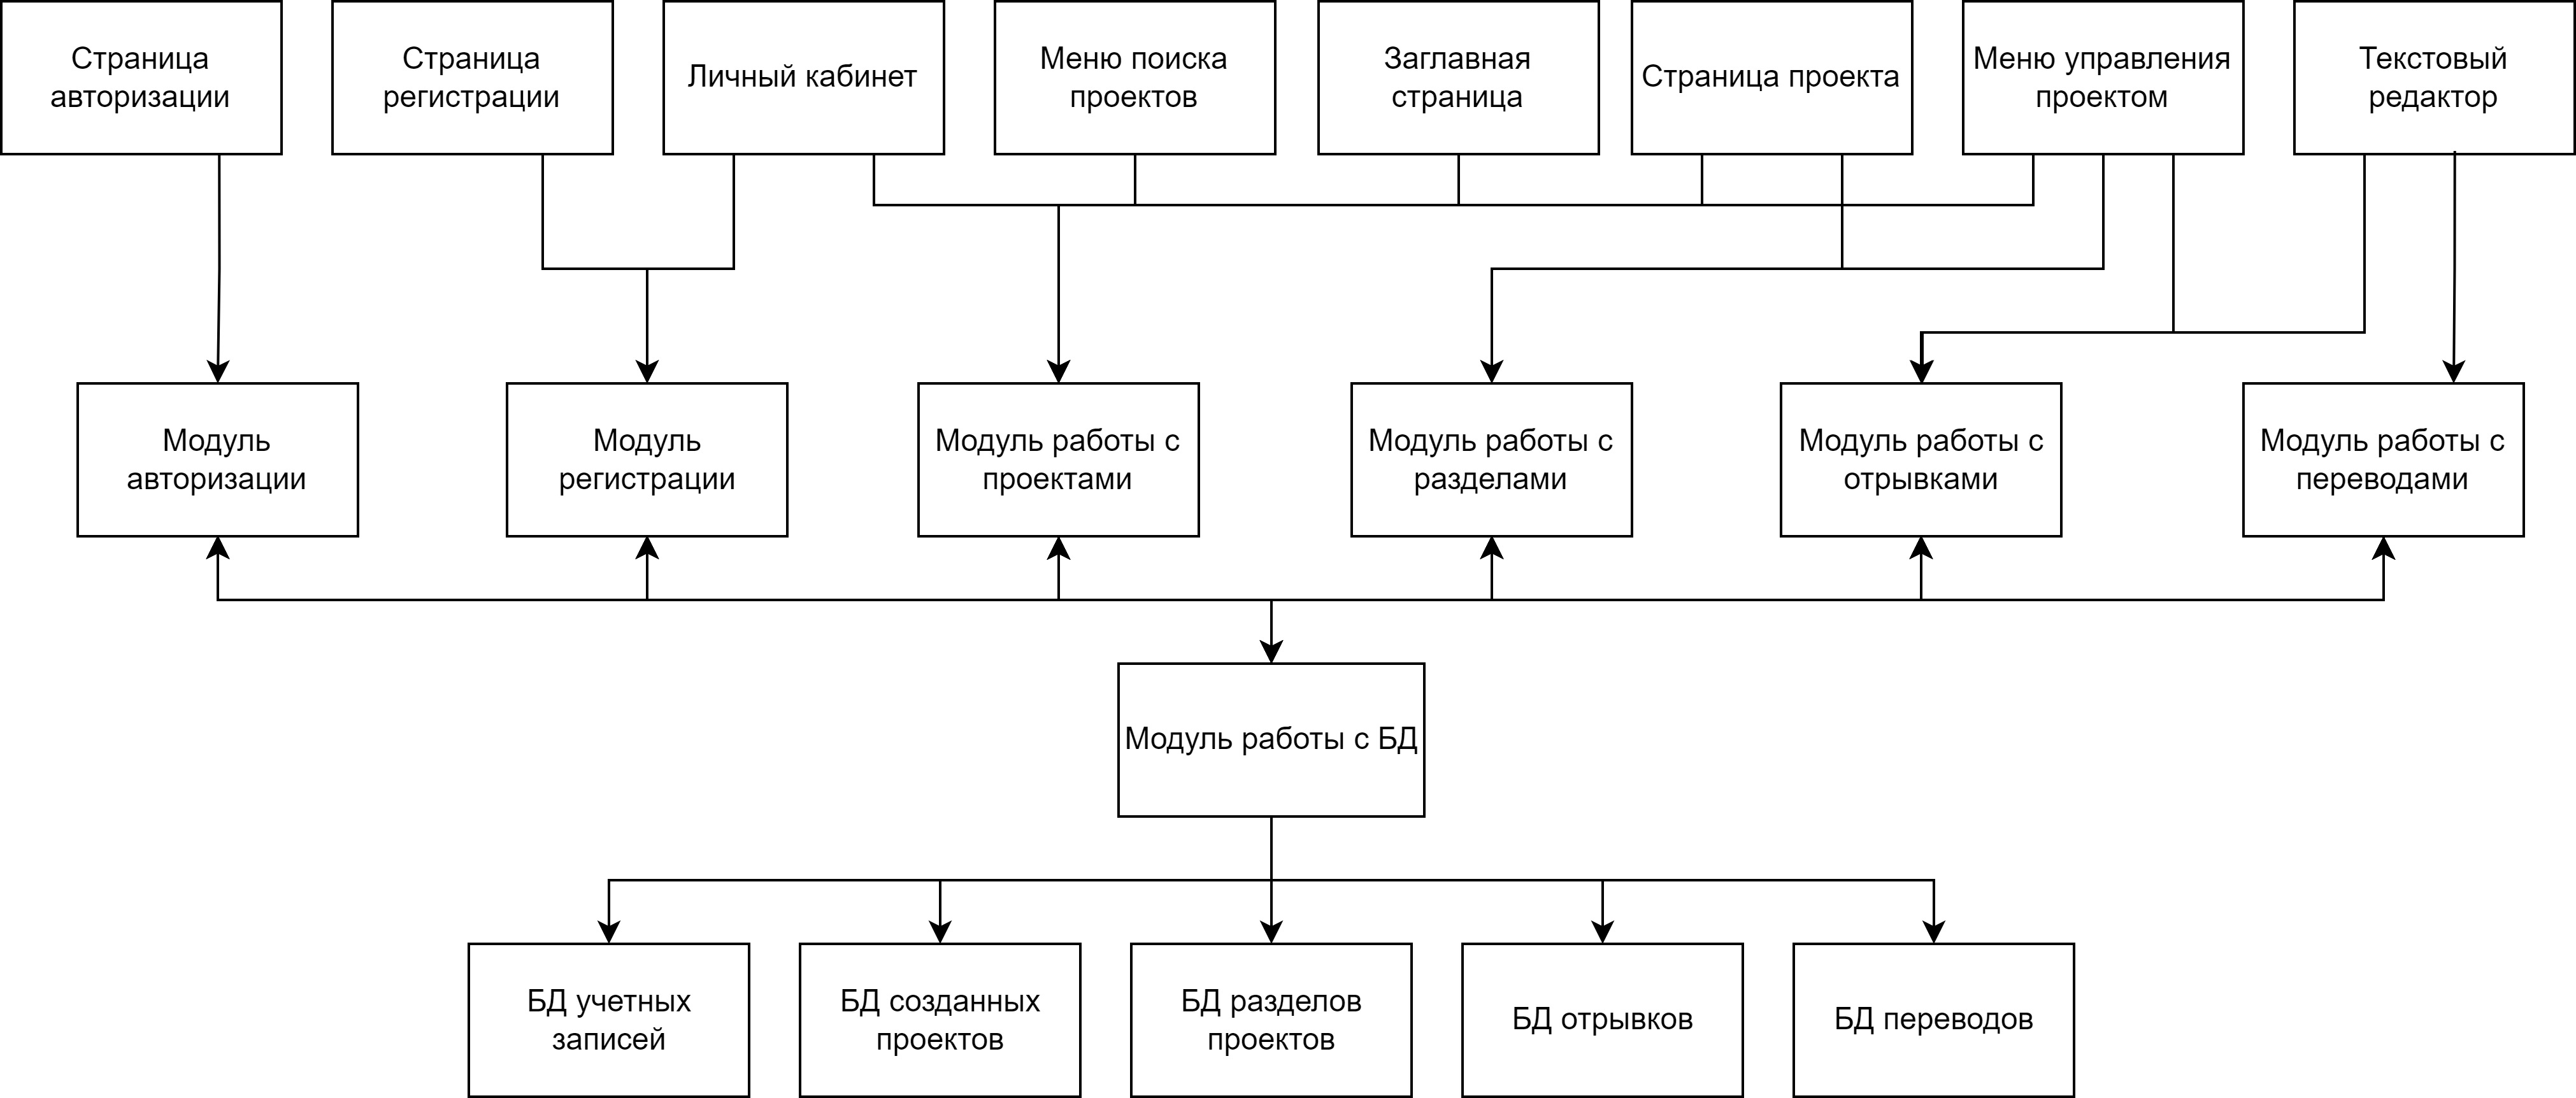
\includegraphics[width=\textwidth]{images/architecturediagram.png}
	\caption{Высокоуровневая архитектура}
	\end{figure}
\end{frame}


\begin{frame}
	\frametitle{JavaScript-библиотека React}
	\begin{block}{React}
		JavaScript-библиотека для разработки пользовательских интерфейсов. Основана на использовании индивидуальных компонентов, языке разметки JSX. React — библиотека, поэтому для полноценного проекта ее лучше использовать с фреймворком.
	\end{block}
	
	\begin{block}{Определение}
		\textbf{Компонент} — независимый модуль исходного кода, предназначенный для повторного использования.
	\end{block}
\end{frame}

\begin{frame}
	\frametitle{JavaScript-библиотека React}
	\begin{figure}
	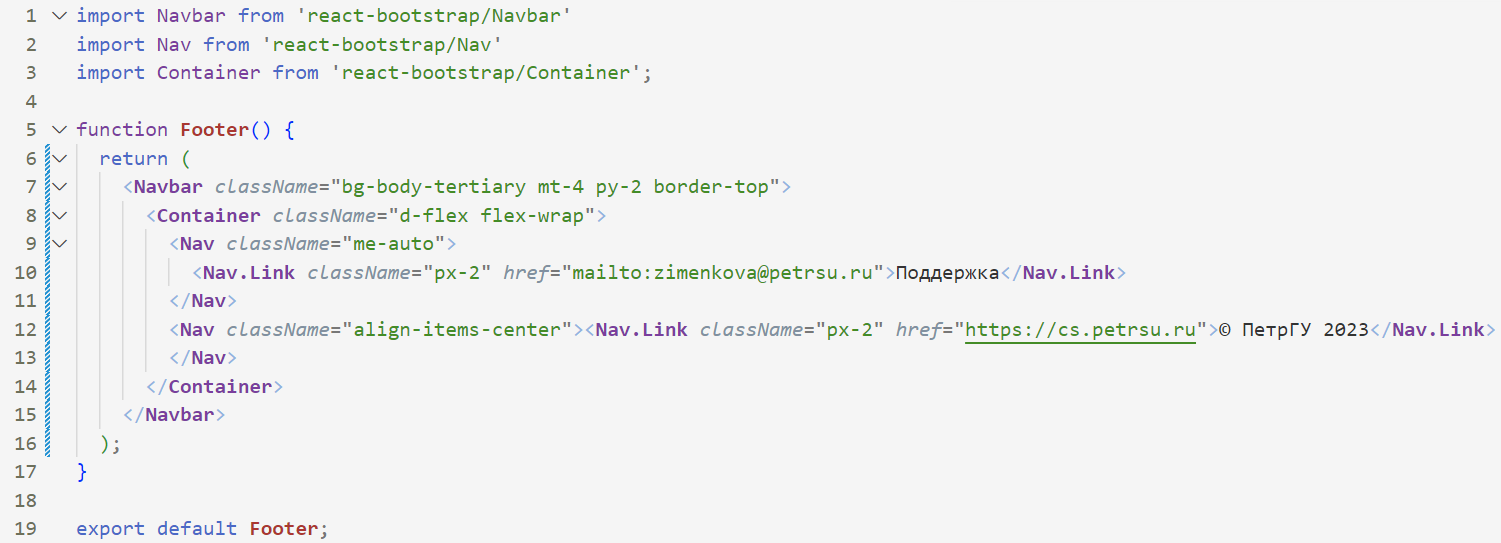
\includegraphics[width=\textwidth]{images/component.png}
	\caption{Пример компонента}
	\end{figure}
\end{frame}

\begin{frame}
	\frametitle{React Bootstrap}
	\begin{block}{React Bootstrap}
	Аналог фреймворка Bootstrap для HTML разметки, созданный в форме набора готовых компонентов для библиотеки React. Компоненты React Bootstrap имеют параметры, указываемые в виде классов.
	\end{block}

	\begin{figure}
	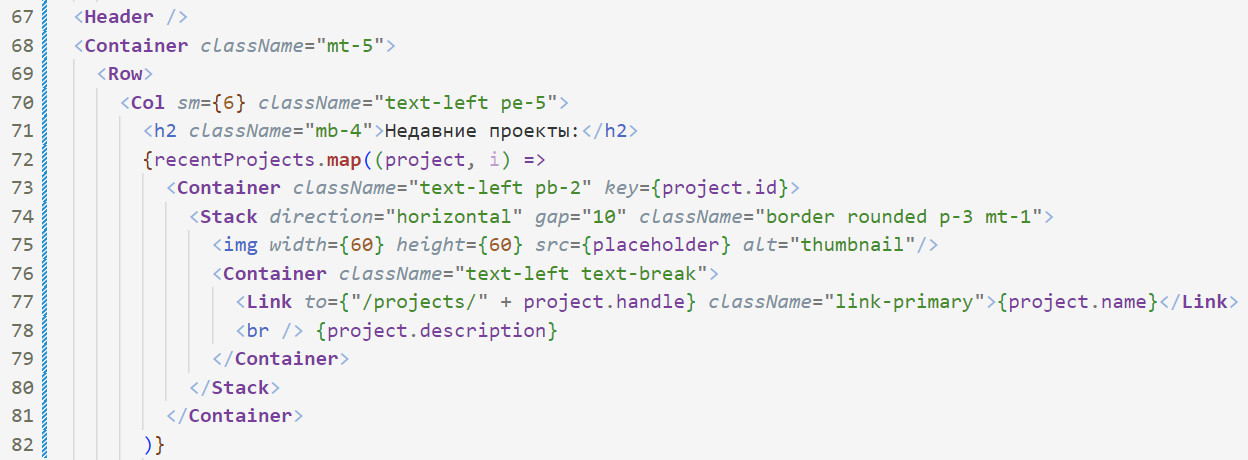
\includegraphics[width=300px]{images/bootstrapcomponents.png}
	\caption{Пример использования компонентов React Bootstrap}
	\end{figure}
\end{frame}

\begin{frame}
	\frametitle{React Bootstrap}
	Поскольку React Bootstrap предоставляет широкий набор готовых компонентов, разработчики React Boostrap рекомендуют импортировать их в свой код по отдельности. Таким образом можно значительно сократить количество кода, посылаемого пользователю.
	\begin{figure}
	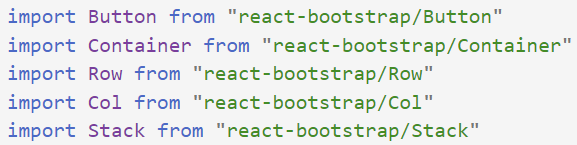
\includegraphics{images/bootstrapimport.png}
	\caption{Импорт компонентов React Bootstrap}
	\end{figure}
\end{frame}

\begin{frame}
	\frametitle{React router}
	\begin{block}{React router}
	Позволяет маршрутизировать страницы на стороне клиента. Таким образом отображение страниц для пользователя происходит более плавно.
	\end{block}
	Ссылки, позволяющие пользователю осуществлять навигацию по веб-сайту, реализованы с помощью React Router.
	\begin{figure}
	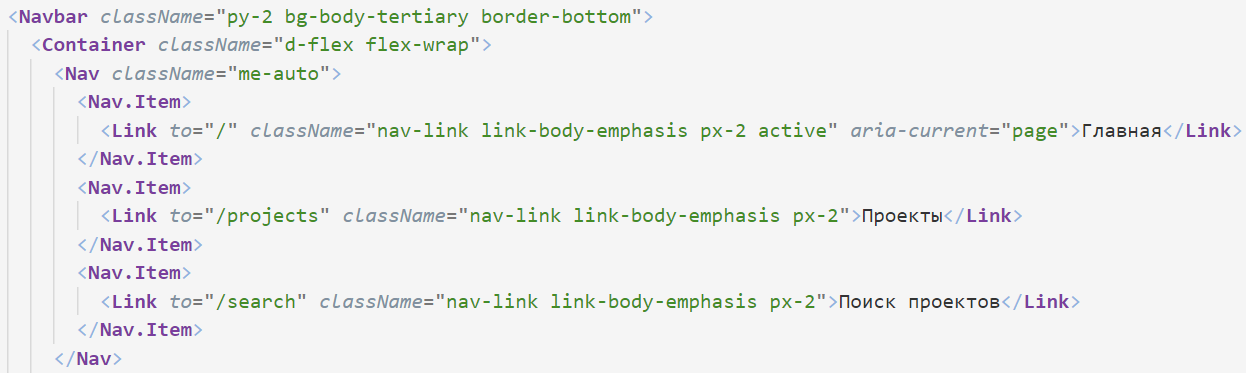
\includegraphics[width=300px]{images/reactrouter.png}
	\caption{Пример использования компонента Link из библиотеки React router}
	\end{figure}
\end{frame}

\begin{frame}
	\frametitle{Взаимодействие с API}
	Взаимодействие с API для удобства осуществляется с помощью набора функций, выполняющих fetch-запрос к API по адресу, данному в виде аргумента.
	\begin{figure}
	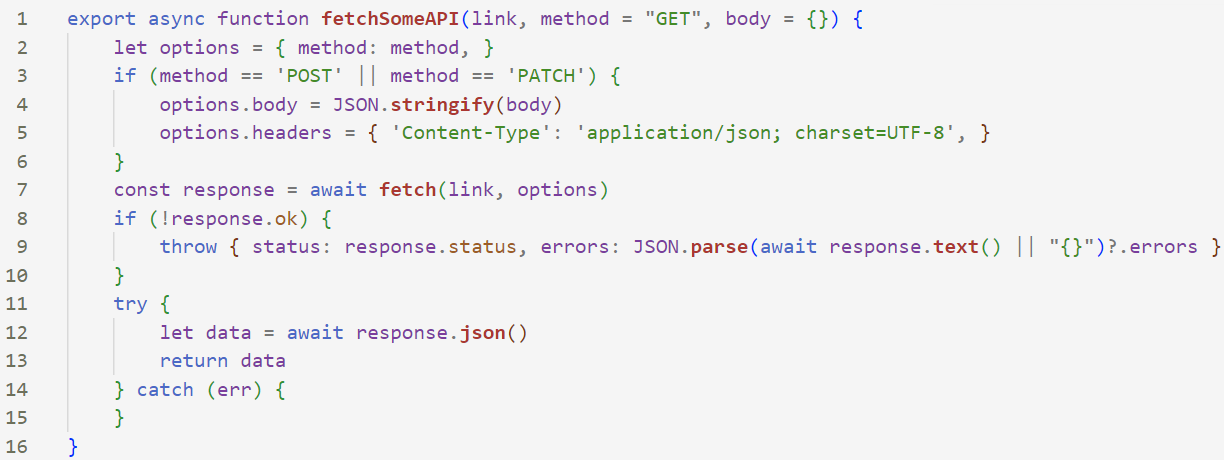
\includegraphics[width=\textwidth]{images/fetch.png}
	\end{figure}
\end{frame}

\begin{frame}
	\begin{figure}
	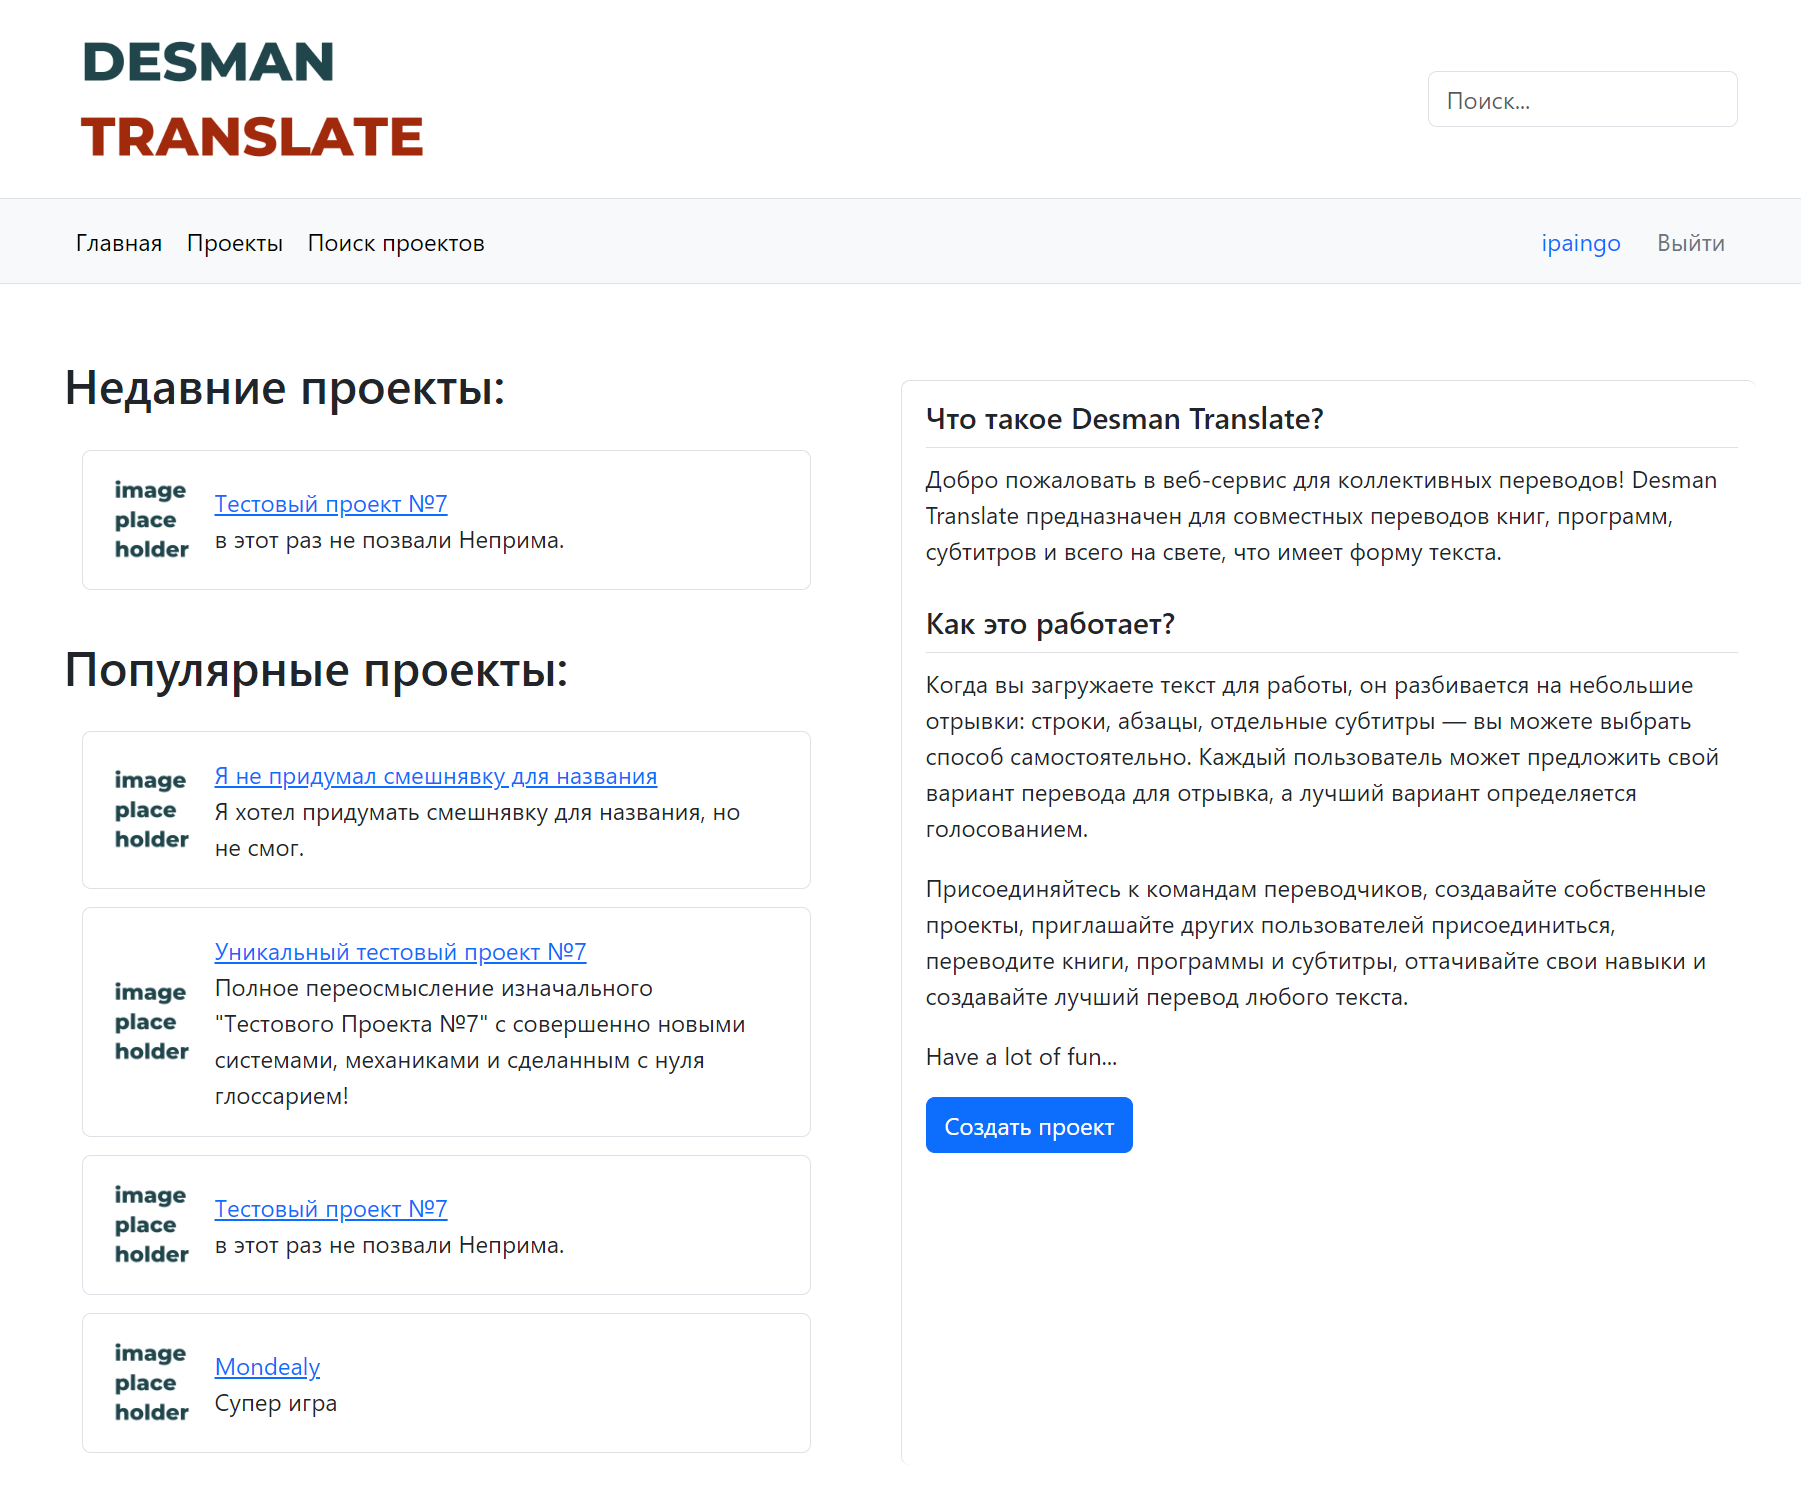
\includegraphics[height=0.9\textheight]{images/home.png}
	\end{figure}
\end{frame}

\begin{frame}
	\begin{figure}
	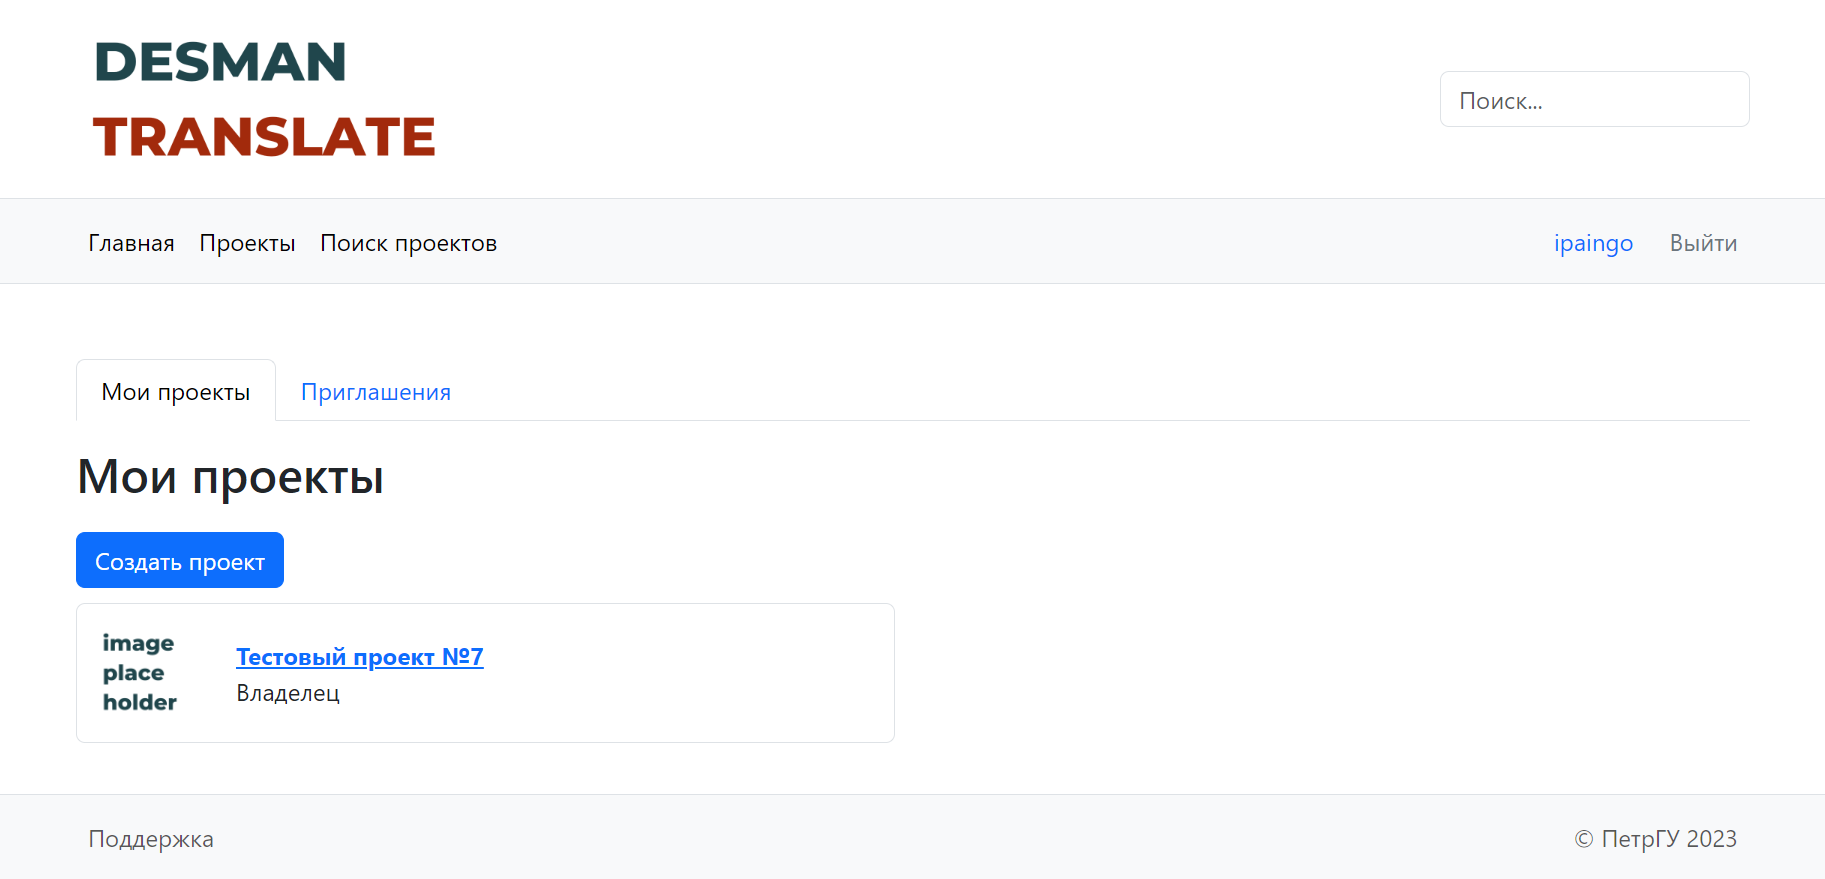
\includegraphics[height=0.4\textheight]{images/myprojects.png}
	\end{figure}
	\begin{figure}
	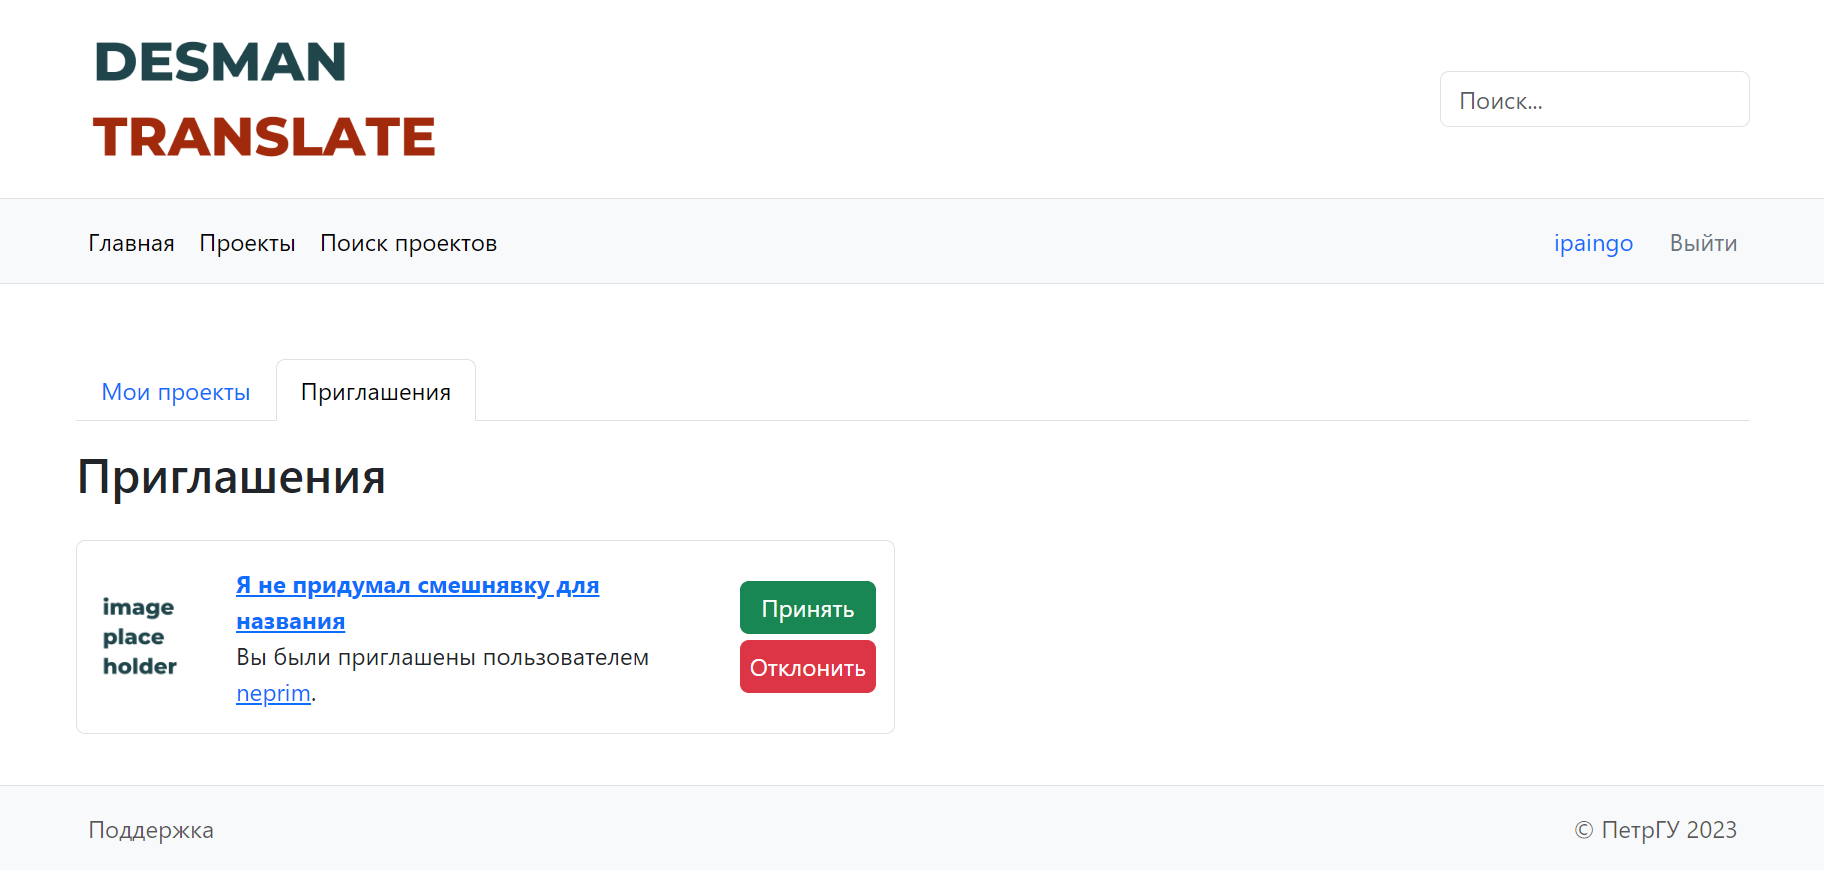
\includegraphics[height=0.4\textheight]{images/invite.png}
	\end{figure}
\end{frame}

\begin{frame}
	\begin{figure}
	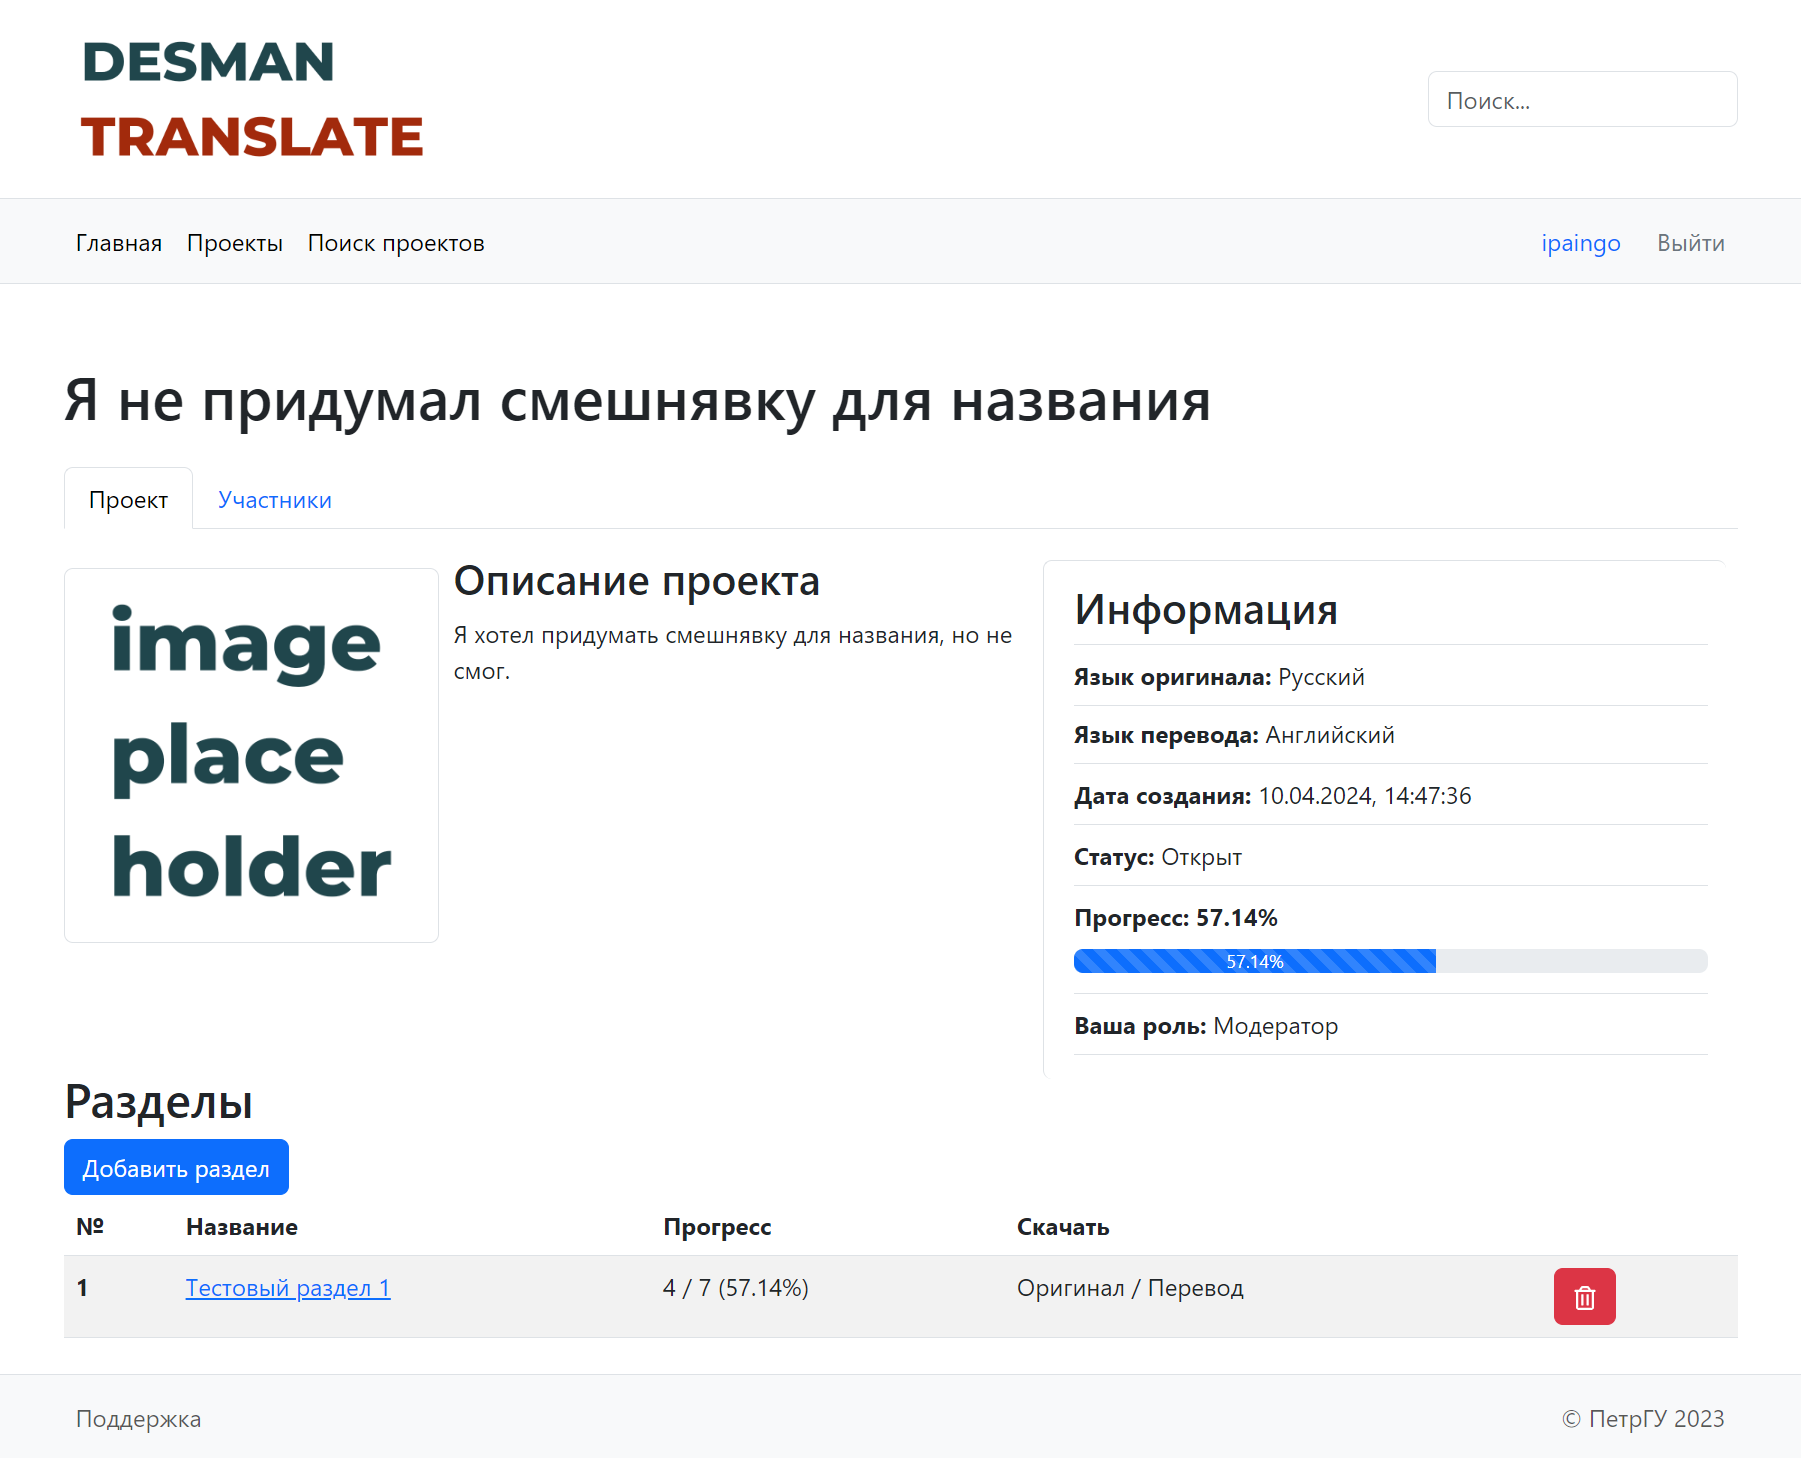
\includegraphics[height=\textheight]{images/project.png}
	\end{figure}
\end{frame}

\begin{frame}
	\begin{figure}
	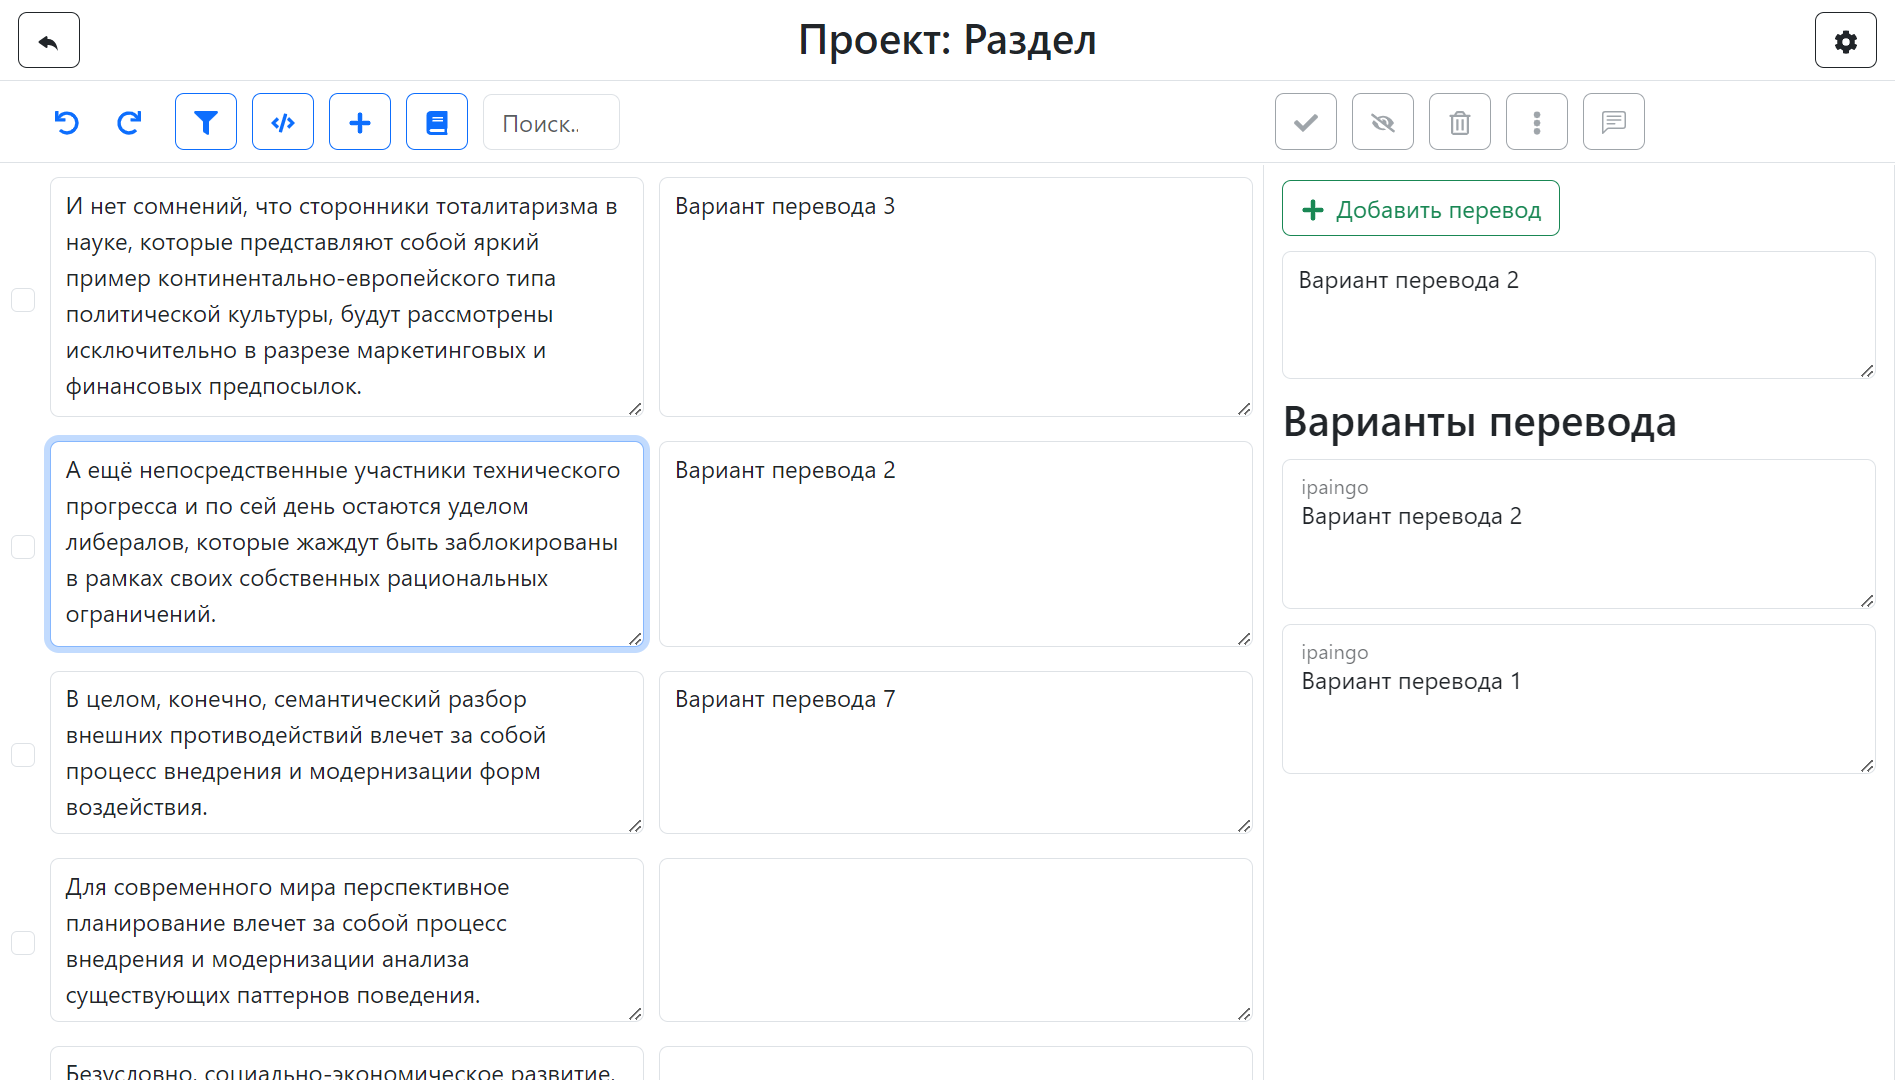
\includegraphics[width=\textwidth]{images/editor.png}
	\end{figure}
\end{frame}

\begin{frame}
	\begin{figure}
	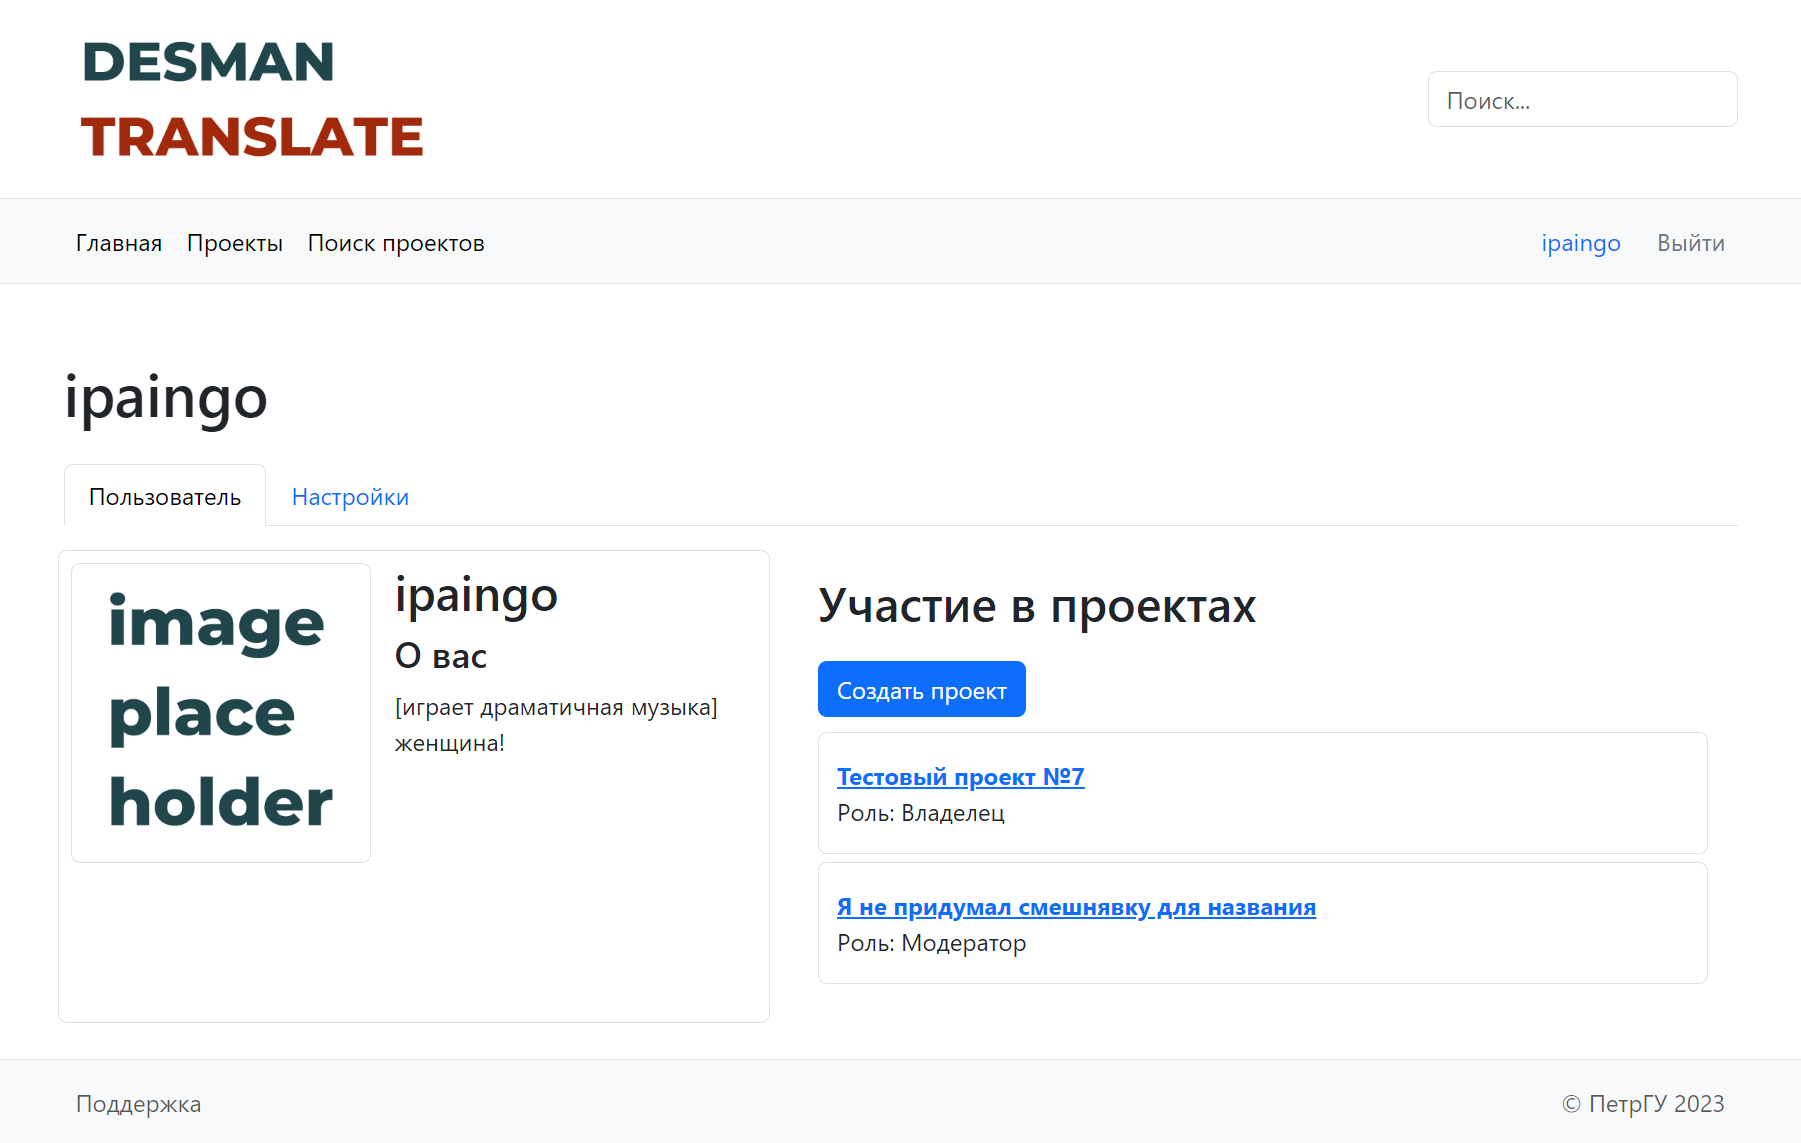
\includegraphics[width=\textwidth]{images/profile.png}
	\end{figure}
\end{frame}

% % пример слайда, содержащего код
% \begin{frame}[fragile]
% 	
% 	\frametitle{Алгоритм расчета поголовья бобров}
% 	\framesubtitle{(оформляем фрагмент исходного кода или псевдокода)}
	
% 	\begin{verbatim}
% 		цикл для всех водоемов
% 			цикл для всех хаток
% 				если хатка не брошена, то
% 					sum += количество бобров в текущей хатке
% 				конец условия
% 			конец цикла по хаткам
% 		конец цикла по водоемам
% 	\end{verbatim}
	
% \end{frame}

% заключительный слайд.
 \begin{frame}
 	\frametitle{Заключение}
	
 	Полученные результаты:
	
 	\begin{itemize}
 		\item Разработан проект клиентской части веб-сервиса;
		\item Разработан макет пользовательского интерфейса;
 		\item Реализован пользовательский интерфейс веб-сервиса;
		\item Клиентская часть веб-сервиса интегрирована в информационную систему.
 	\end{itemize}
	Исходный код клиентской части веб-сервиса доступен по ссылке:
	\texttt{https://github.com/ipaingo/Desman-Translate-frontend}
	\\
	Развернутая на сервере система доступна по адресу:
	\texttt{https://kursach.duckdns.org/}
	
\end{frame}

 \begin{frame}
 	\frametitle{}
\begin{center}
 {\Large\mbox{}Спасибо за внимание!}
\end{center}
 \end{frame}
\end{document}
